%\chapter{Anhang}
\chapter{Anhang}

\begin{figure}[htbp]
	\centering
	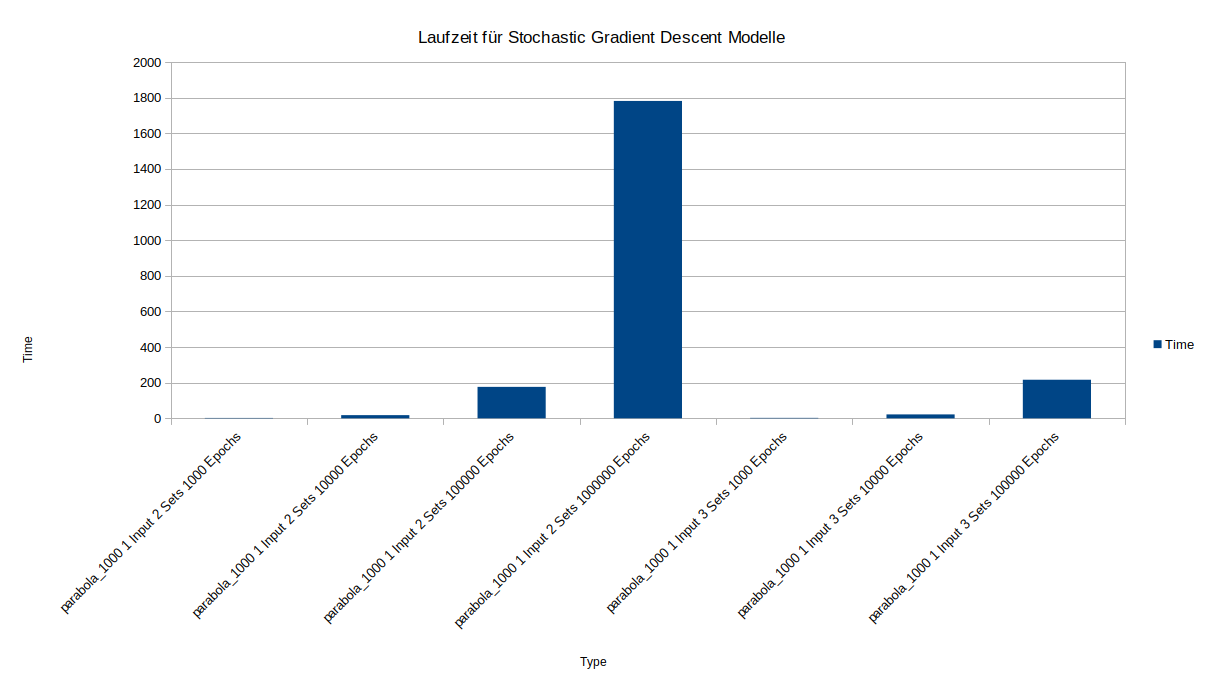
\includegraphics[angle=-90,totalheight=0.66\textheight]{images/charts/StochasticGradientTimeParabola.png}
	\caption{Laufzeit für Stochastic-Modelle beim Erlernen der Parabelfunktion}
\end{figure}

\begin{figure}[htbp]
	\centering
	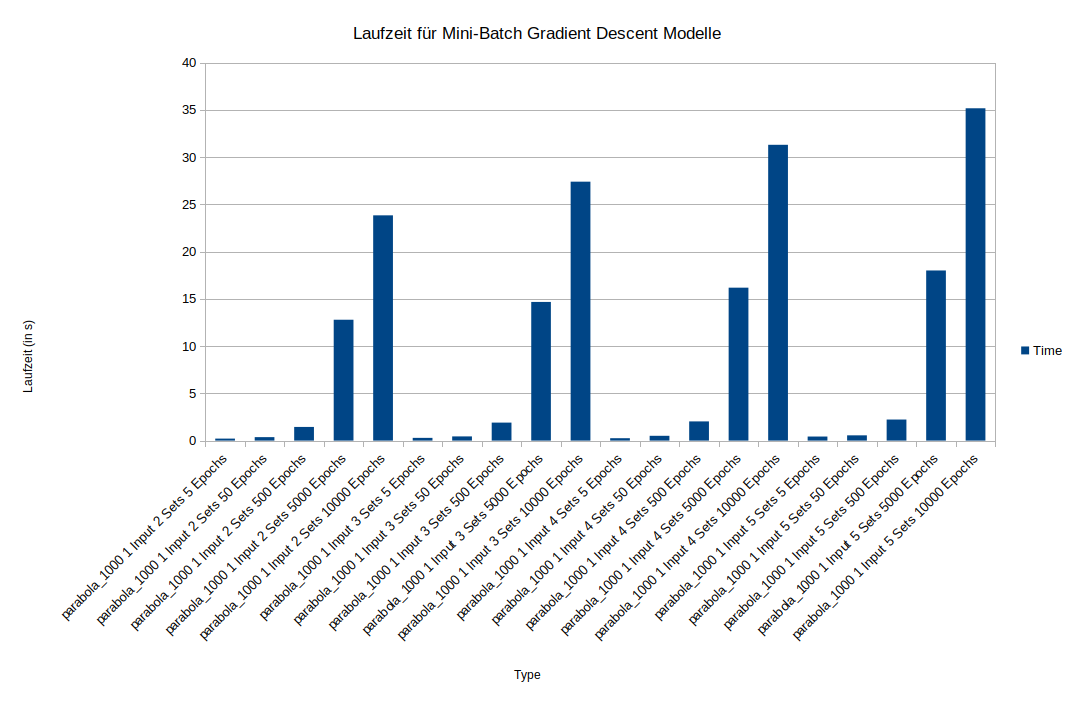
\includegraphics[angle=-90,totalheight=\textheight]{images/charts/Mini-BatchGradientTimeParabola.png}
	\caption{Laufzeit für Mini-Batch-Modelle beim Erlernen der Parabelfunktion}
\end{figure}

\begin{figure}[htbp]
	\centering
	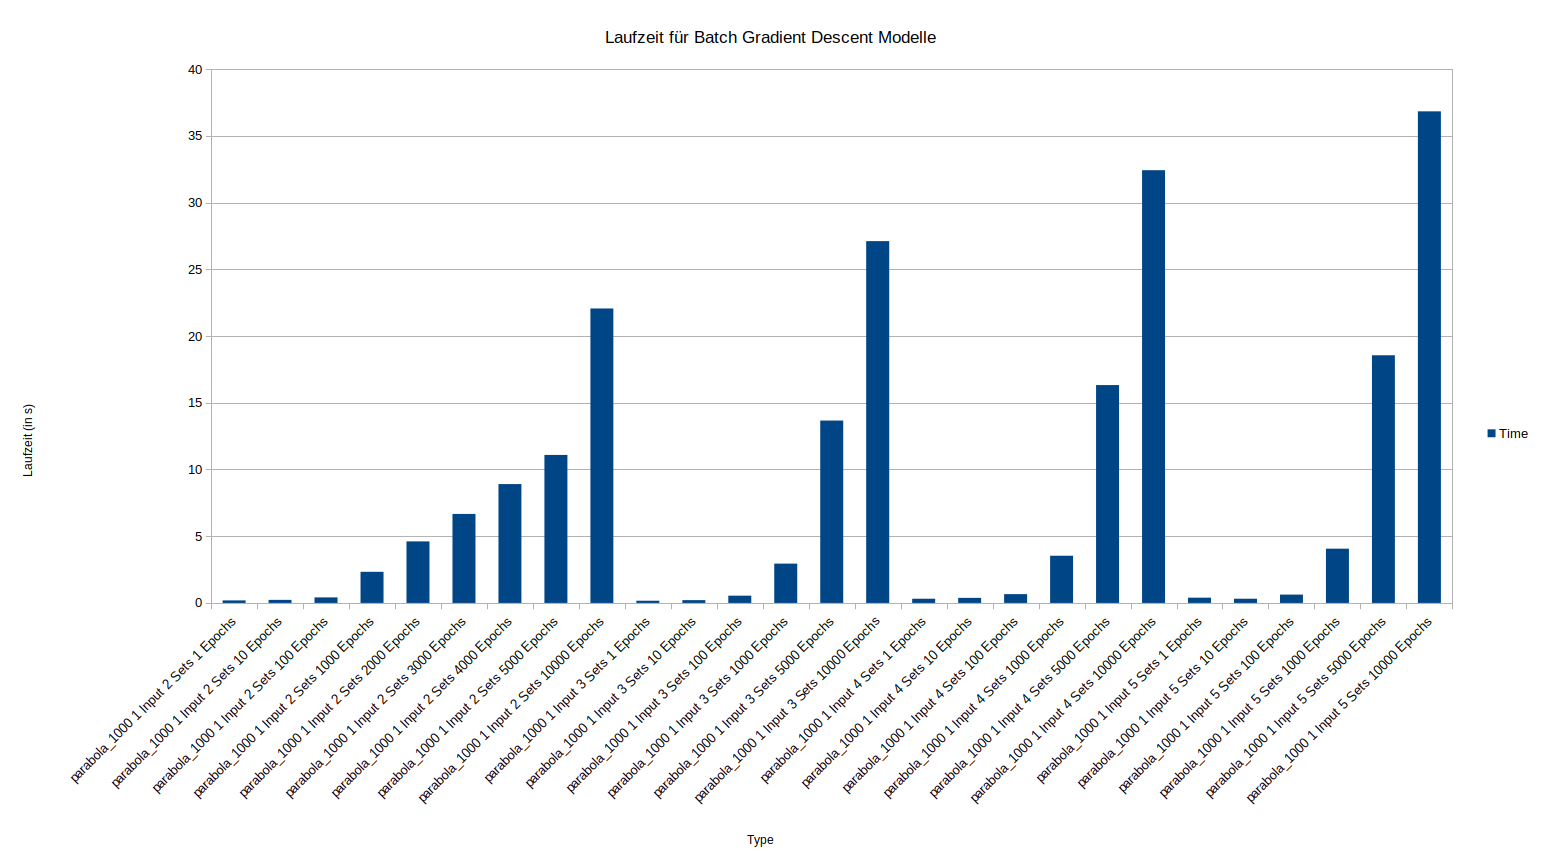
\includegraphics[angle=-90,totalheight=\textheight]{images/charts/BatchGradientTimeParabola.png}
	\caption{Laufzeit für Batch-Modelle beim Erlernen der Parabel Funktion}
\end{figure}

\begin{figure}[htbp]
	\centering
	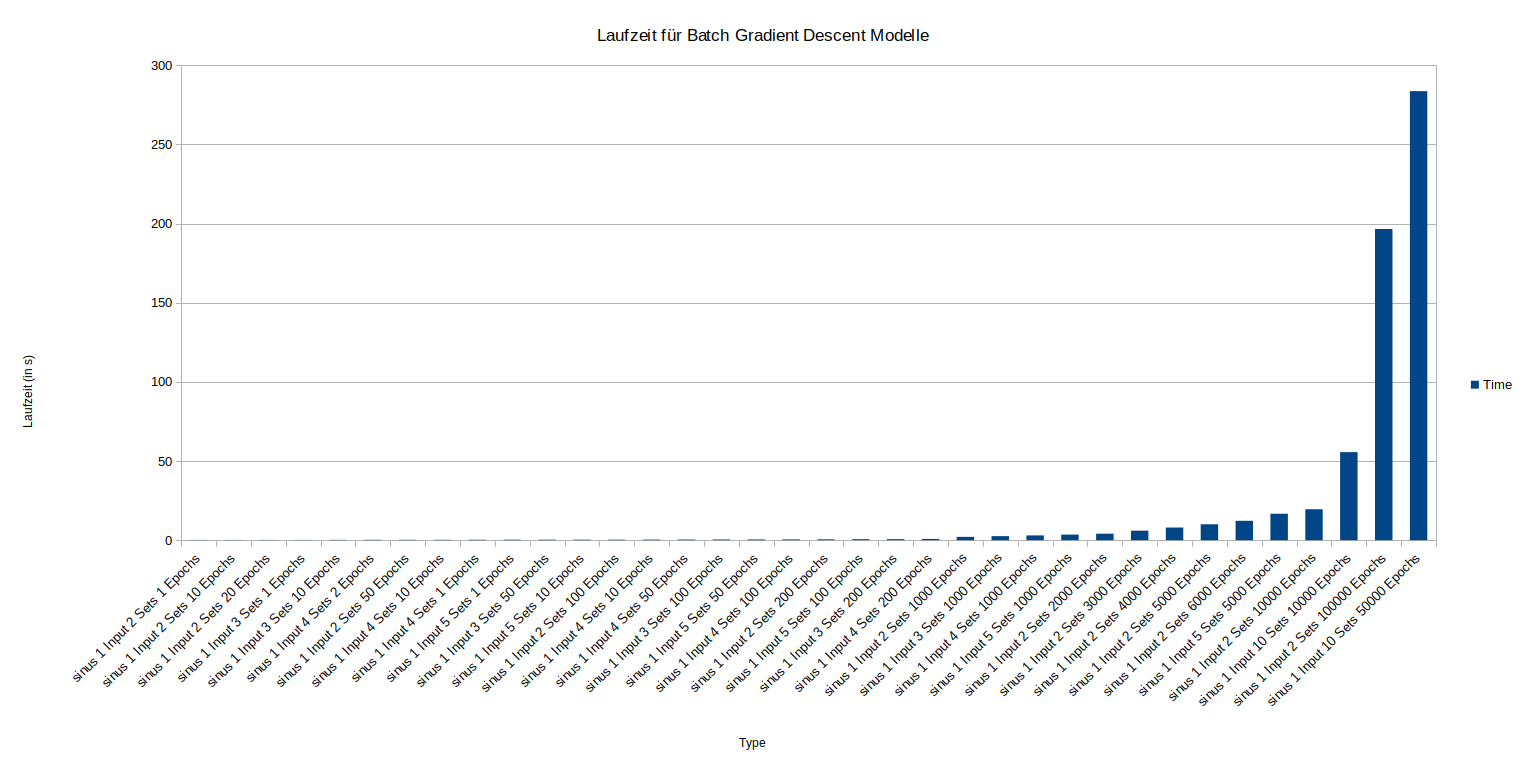
\includegraphics[angle=-90,totalheight=\textheight]{images/charts/BatchGradientTimeSinus.png}
	\caption{Laufzeit für Batch-Modelle beim Erlernen der Sinusfunktion}
\end{figure}

\begin{figure}[htbp]
	\centering
	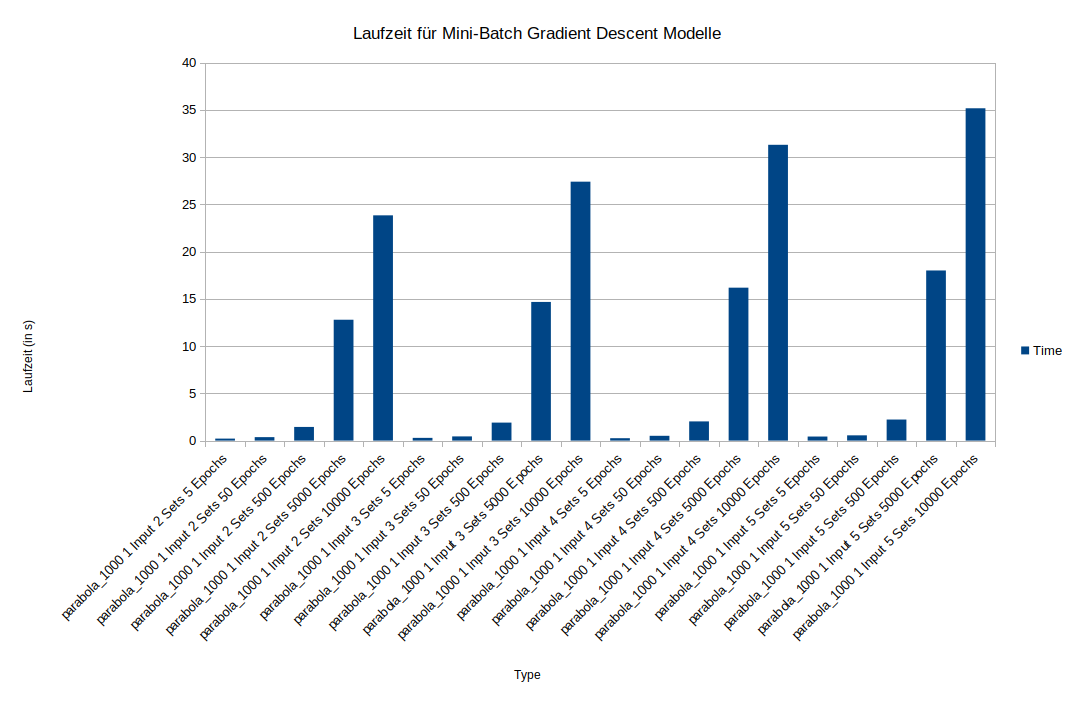
\includegraphics[angle=-90,totalheight=\textheight]{images/charts/Mini-BatchGradientTimeParabola.png}
	\caption{Laufzeit für Mini-Batch-Modelle beim Erlernen der Parabelfunktion}
\end{figure}

\begin{figure}[htbp]
	\centering
	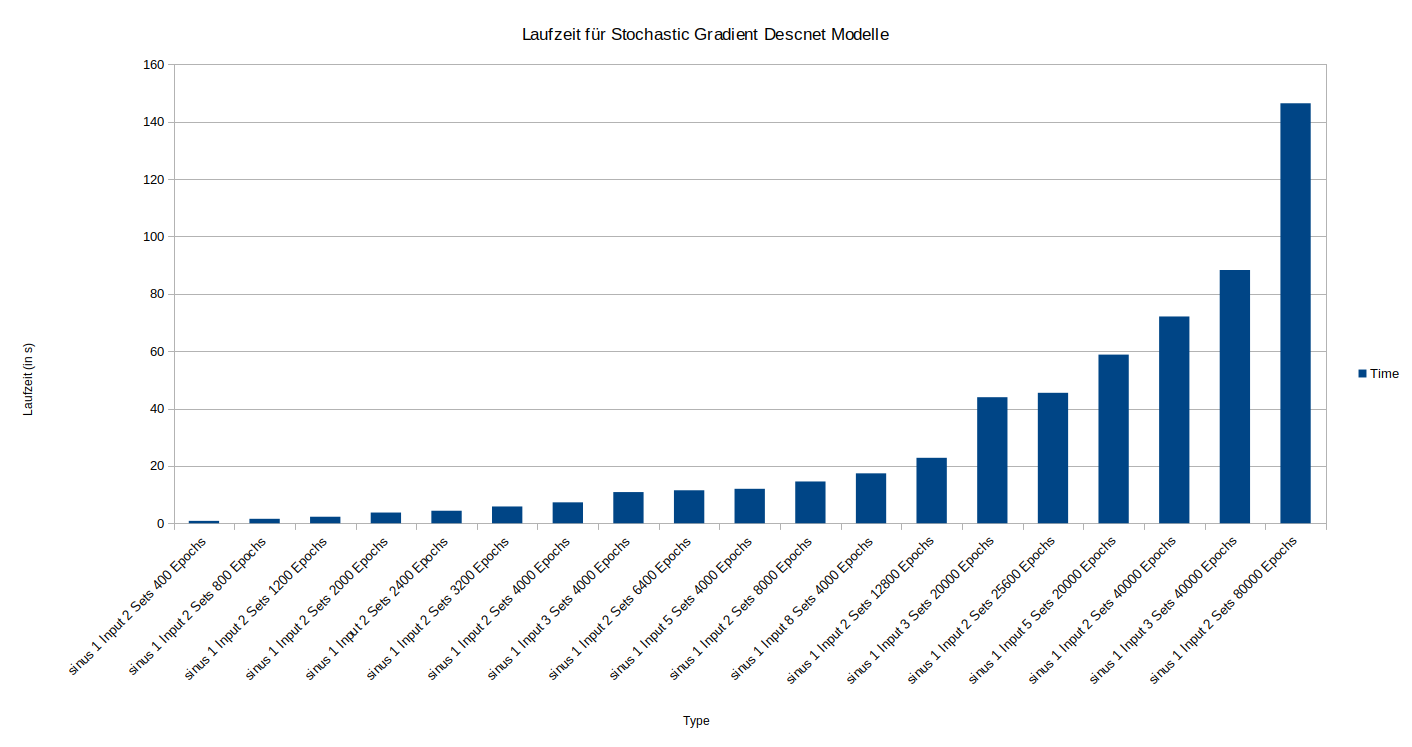
\includegraphics[angle=-90,totalheight=\textheight]{images/charts/StochasticGradientTimeSinus.png}
	\caption{Laufzeit für Stochastic-Modelle beim Erlernen der Sinusfunktion}
\end{figure}